\section{Methods}

\begin{frame}[t, fragile]
    \frametitle{Challenges and Proposed Solution}

    \begin{itemize}
        \item<1-> \textbf{Challenges:}
              \begin{itemize}
                  \item Sparse-view data increases the ill-posedness of the problem.
                  \item Hand-crafted regularizers (e.g., Total Variation) tend to oversmooth and erase subtle image features.
              \end{itemize}

        \item<2-> \textbf{Solution Overview:}
              \begin{itemize}
                  \item JRM via Adaptive Diffusion Models (ADMs).
                  \item Motion-free $\textcolor{green}{\boldx}$ is estimated via a Deep Posterior Sampling (DPS) approach \cite{zhu2023denoising}.
                  \item Motion parameters $\textcolor{orange}{\boldphi}, \textcolor{orange}{\bolds}$ are estimated through a classical optimization pipeline.
                  \item Wavelet Diffusion Models (WDMs) \cite{friedrich2024wdm} are used to enhance computational efficiency.
              \end{itemize}
    \end{itemize}
\end{frame}



\begin{frame}[fragile]
	\frametitle{Overview of JRM-ADM}
	
        \only<1>{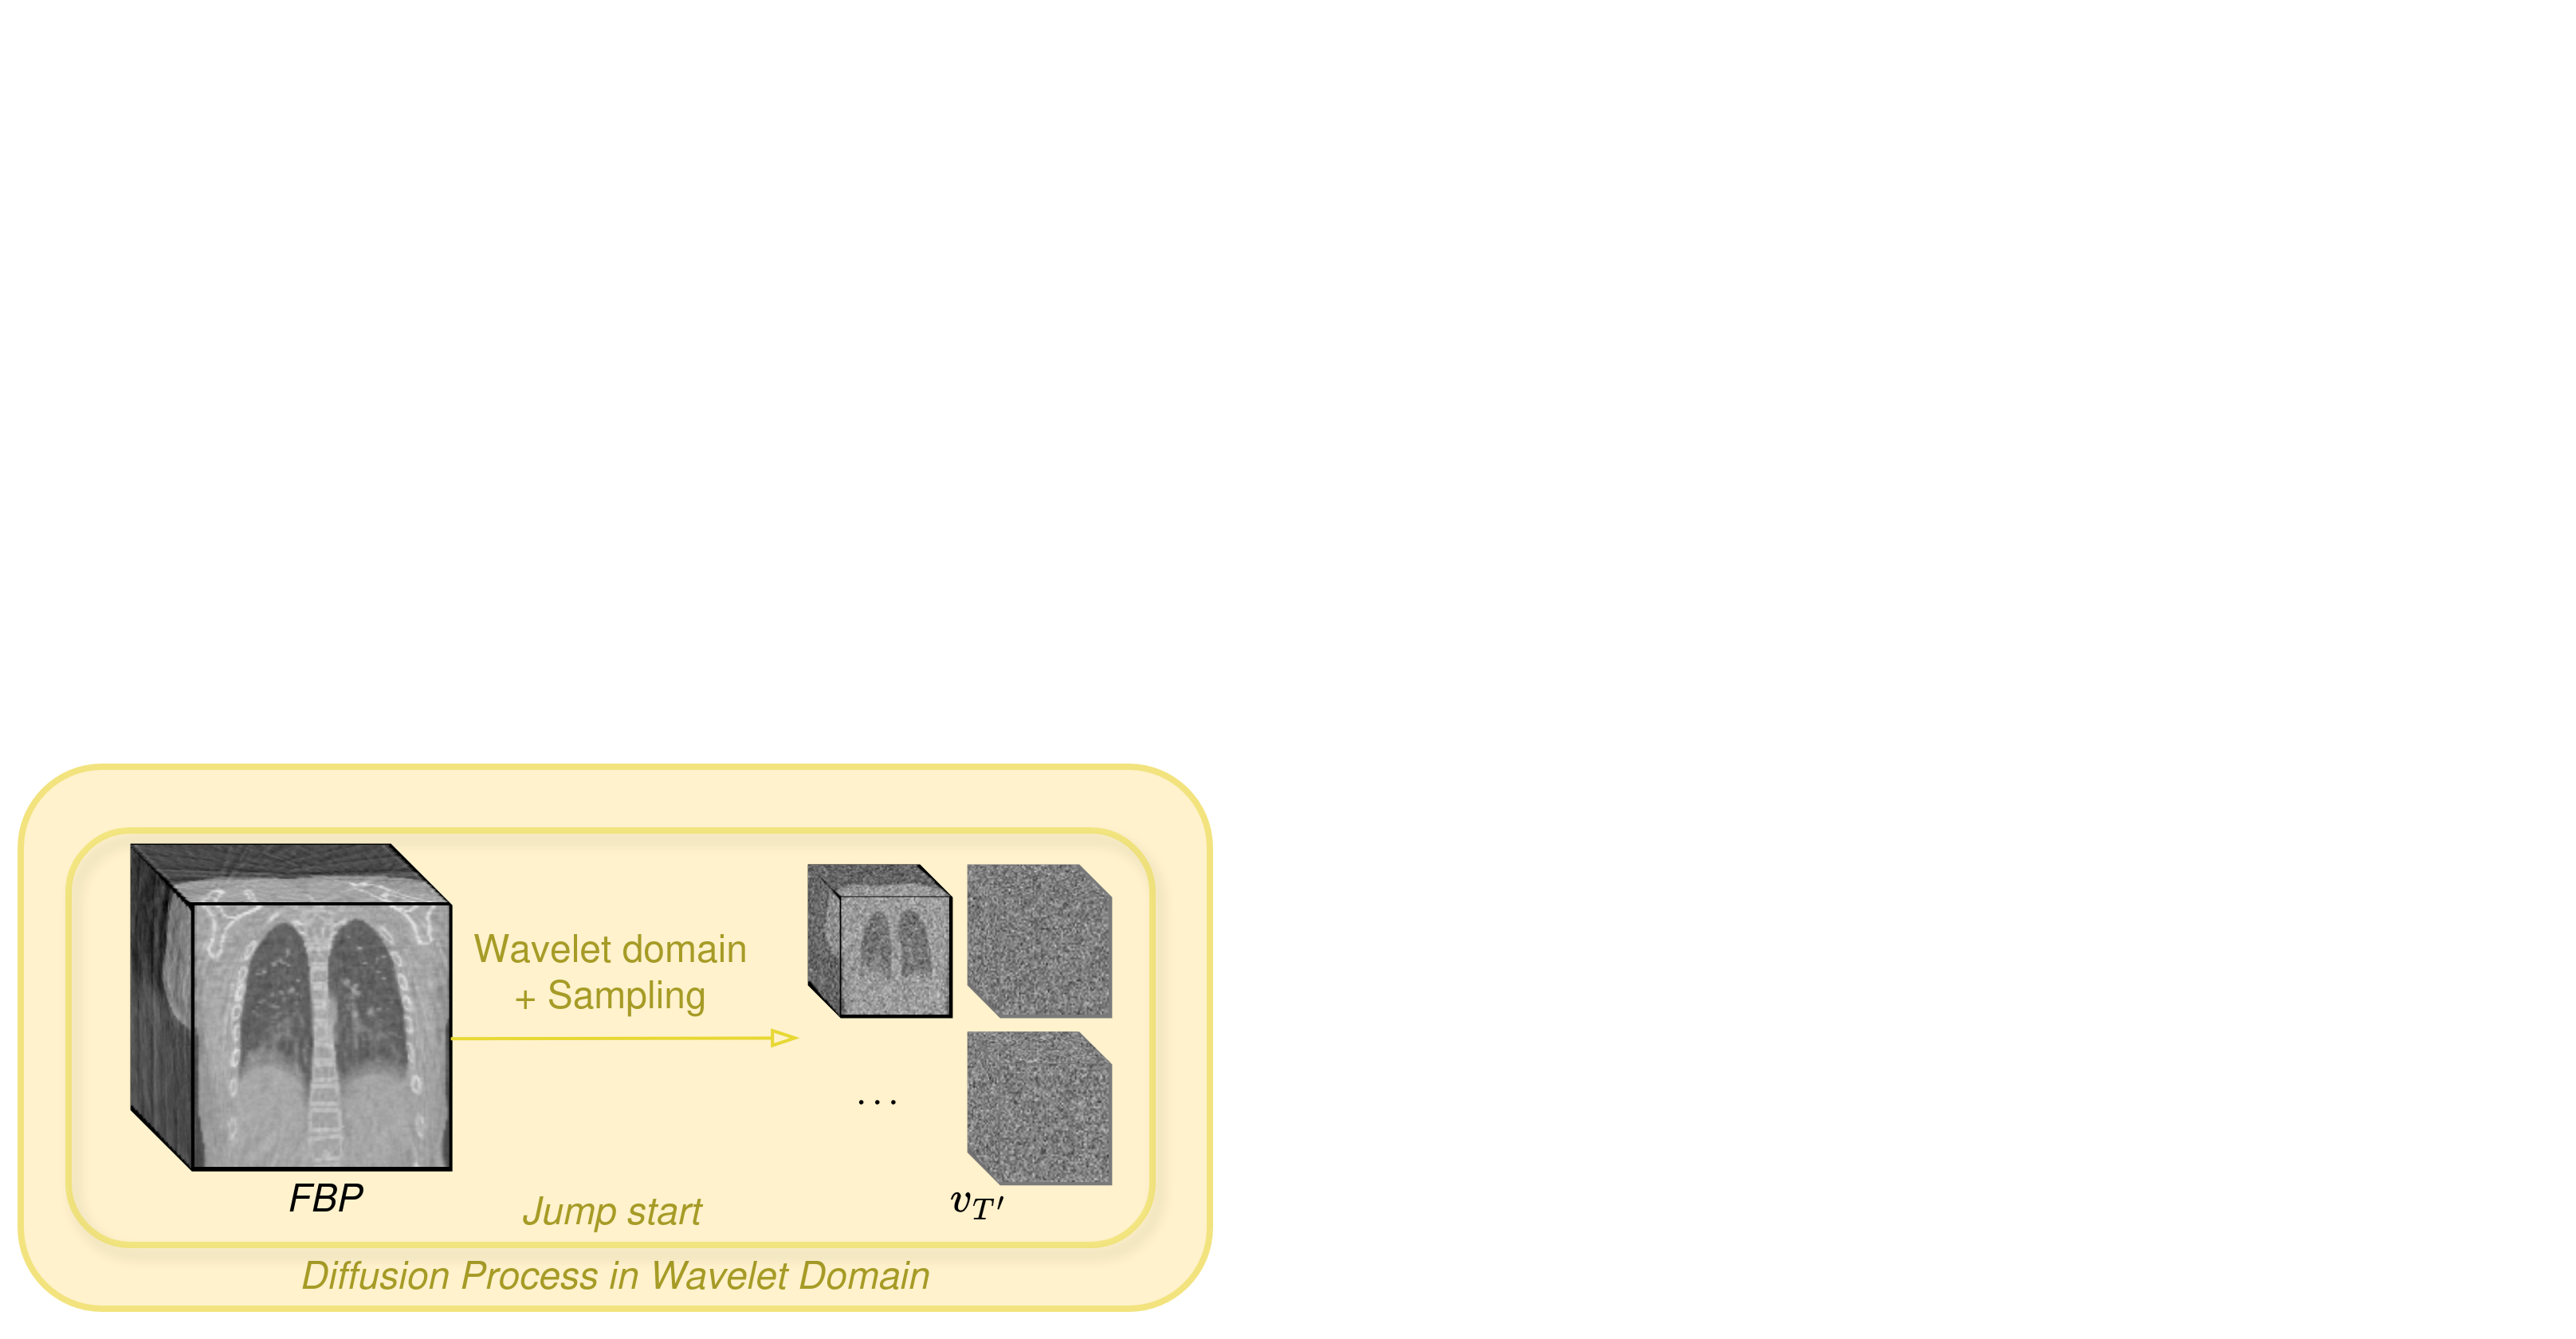
\includegraphics[width=1.0\linewidth]{figures/methods/overview/overview_1.png}}
        \only<2>{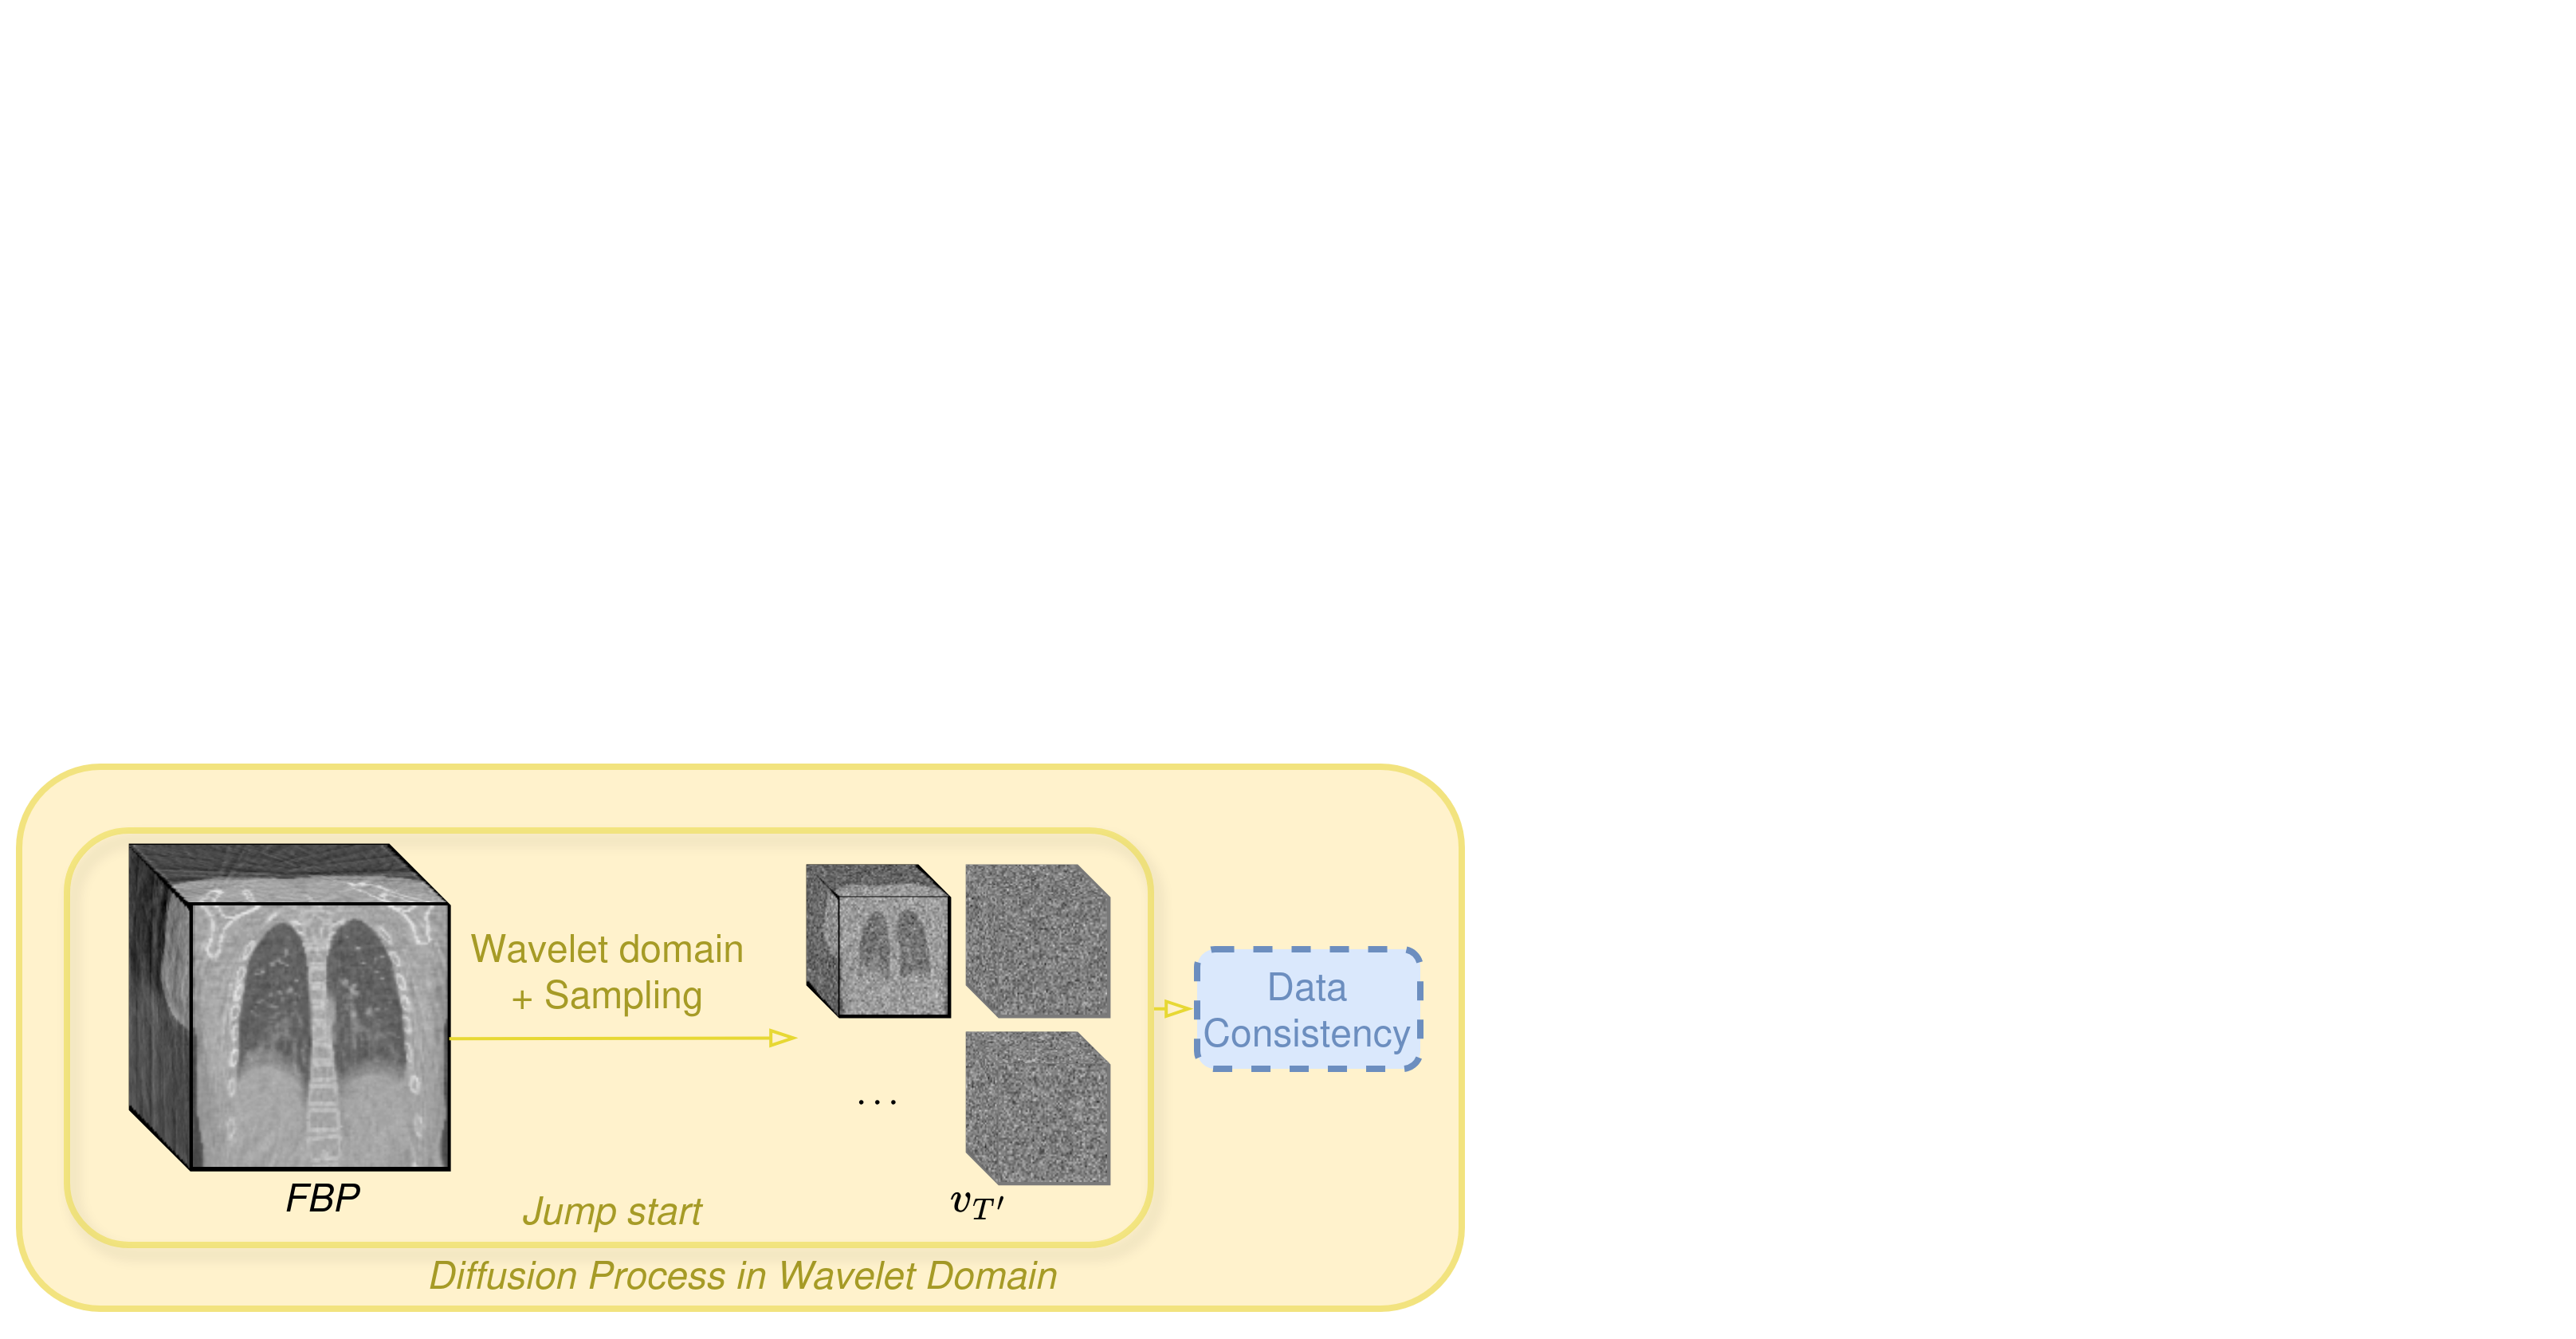
\includegraphics[width=1.0\linewidth]{figures/methods/overview/overview_2.png}}
        \only<3>{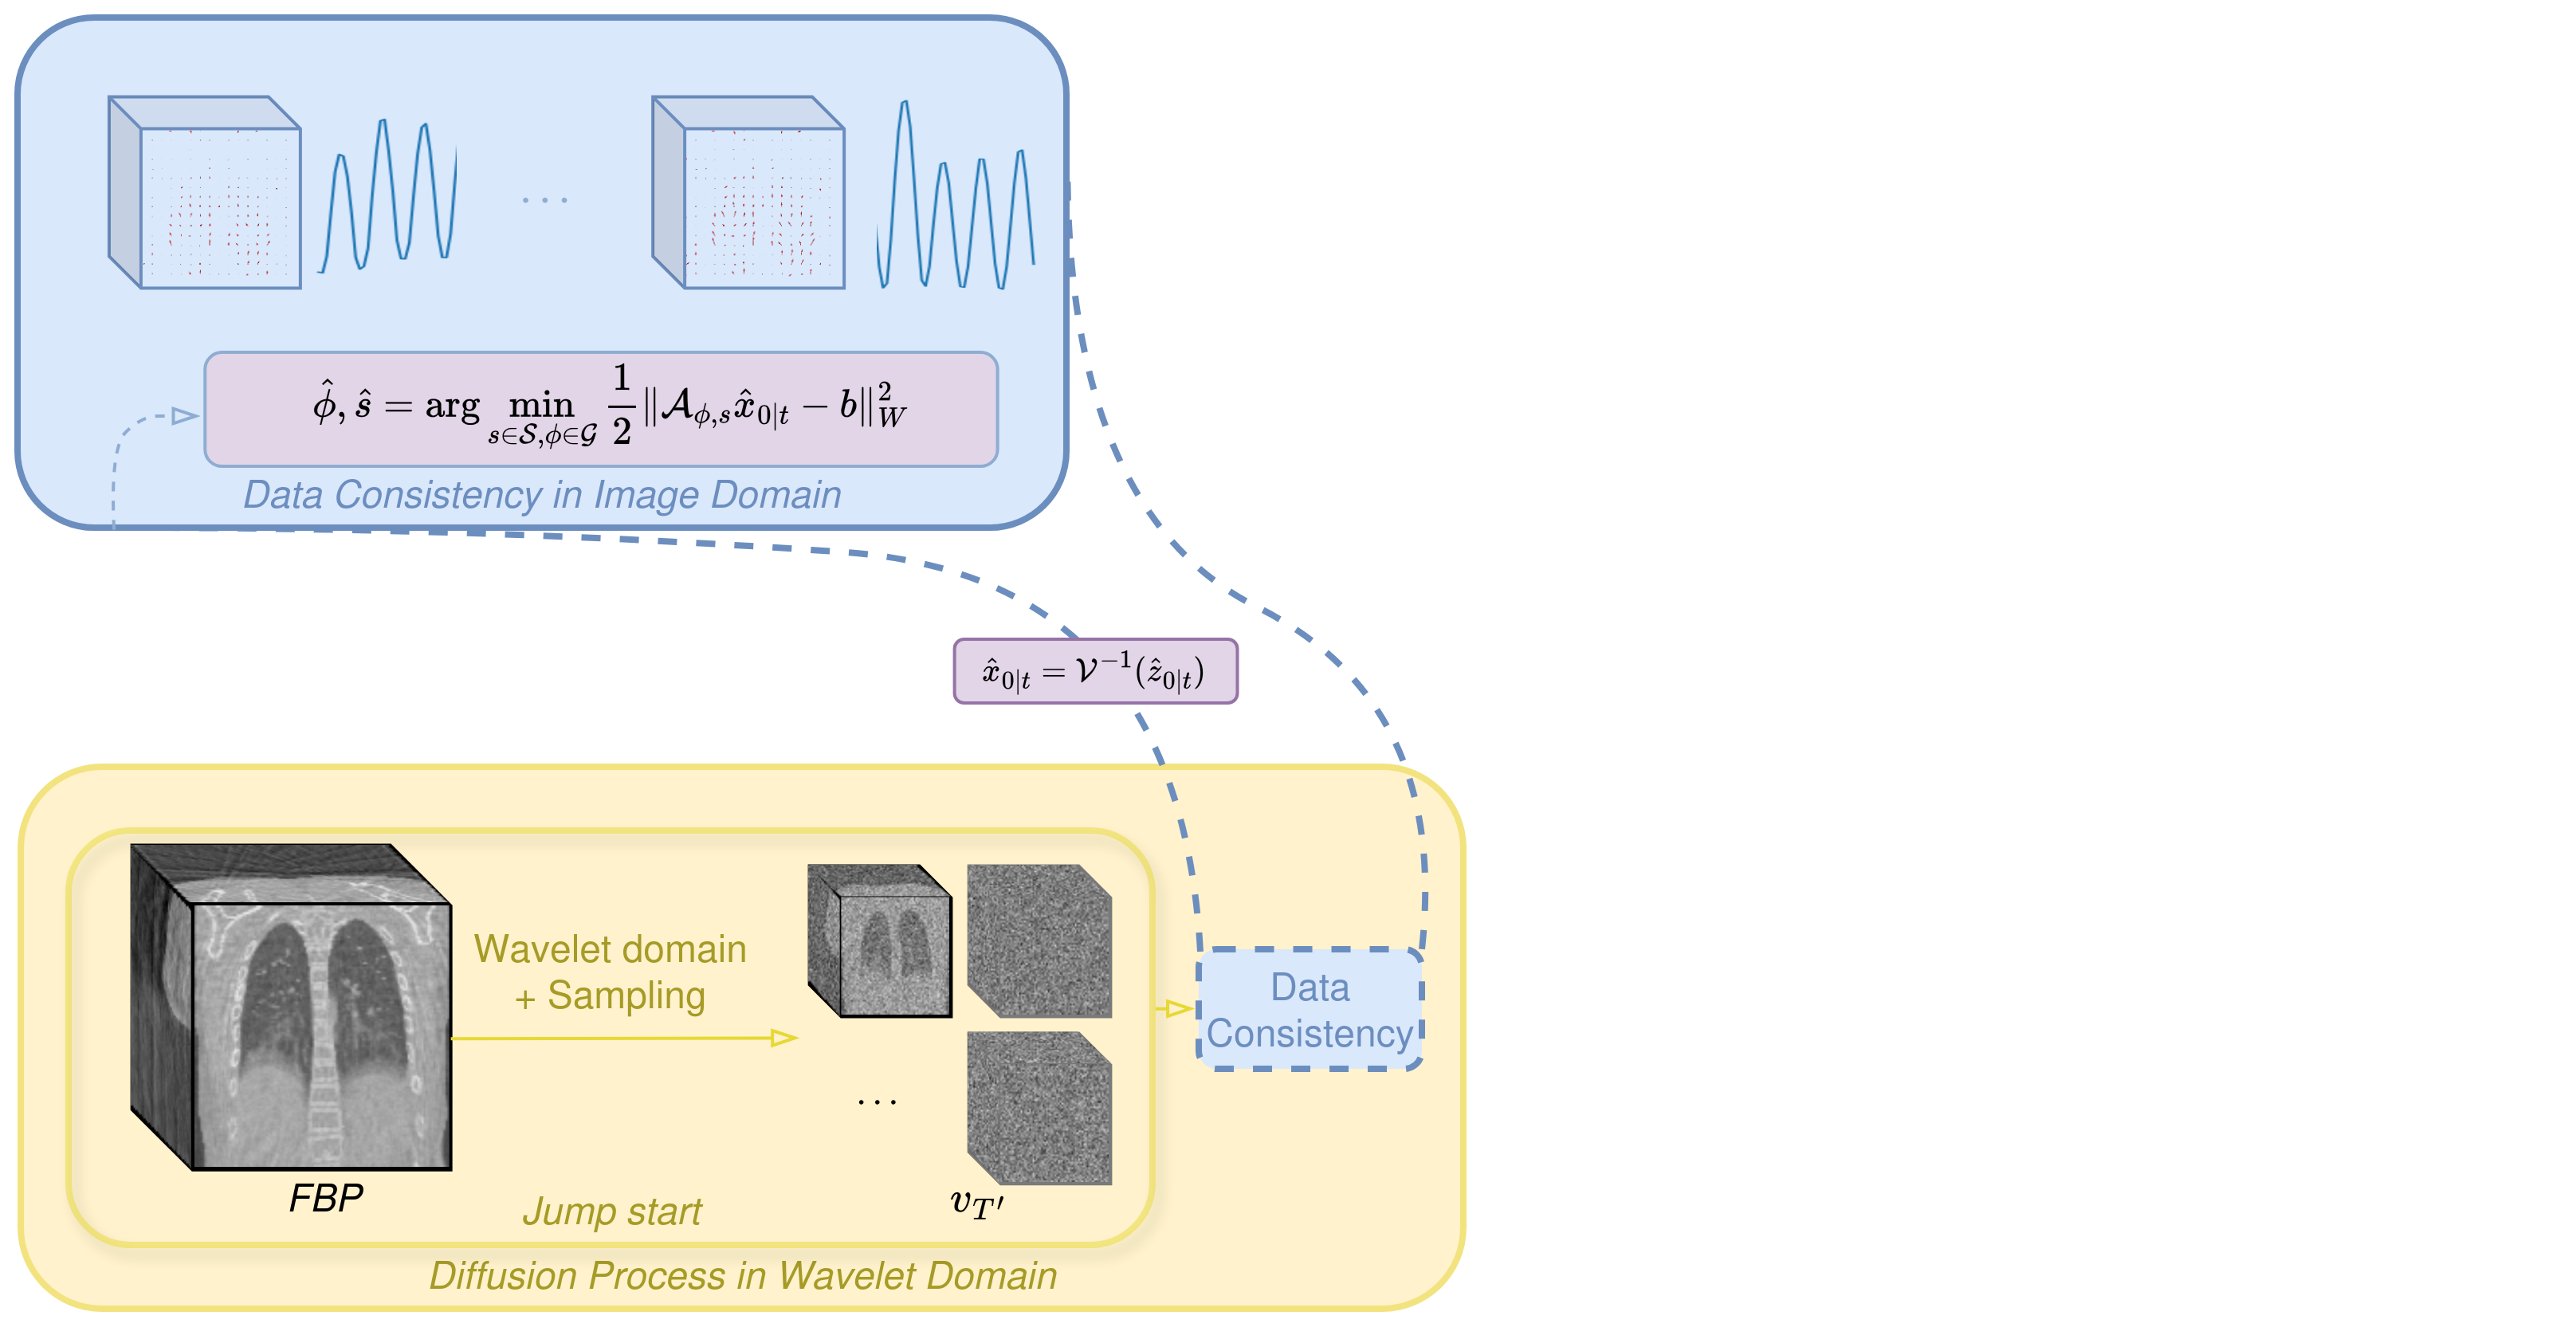
\includegraphics[width=1.0\linewidth]{figures/methods/overview/overview_3.png}}
        \only<4>{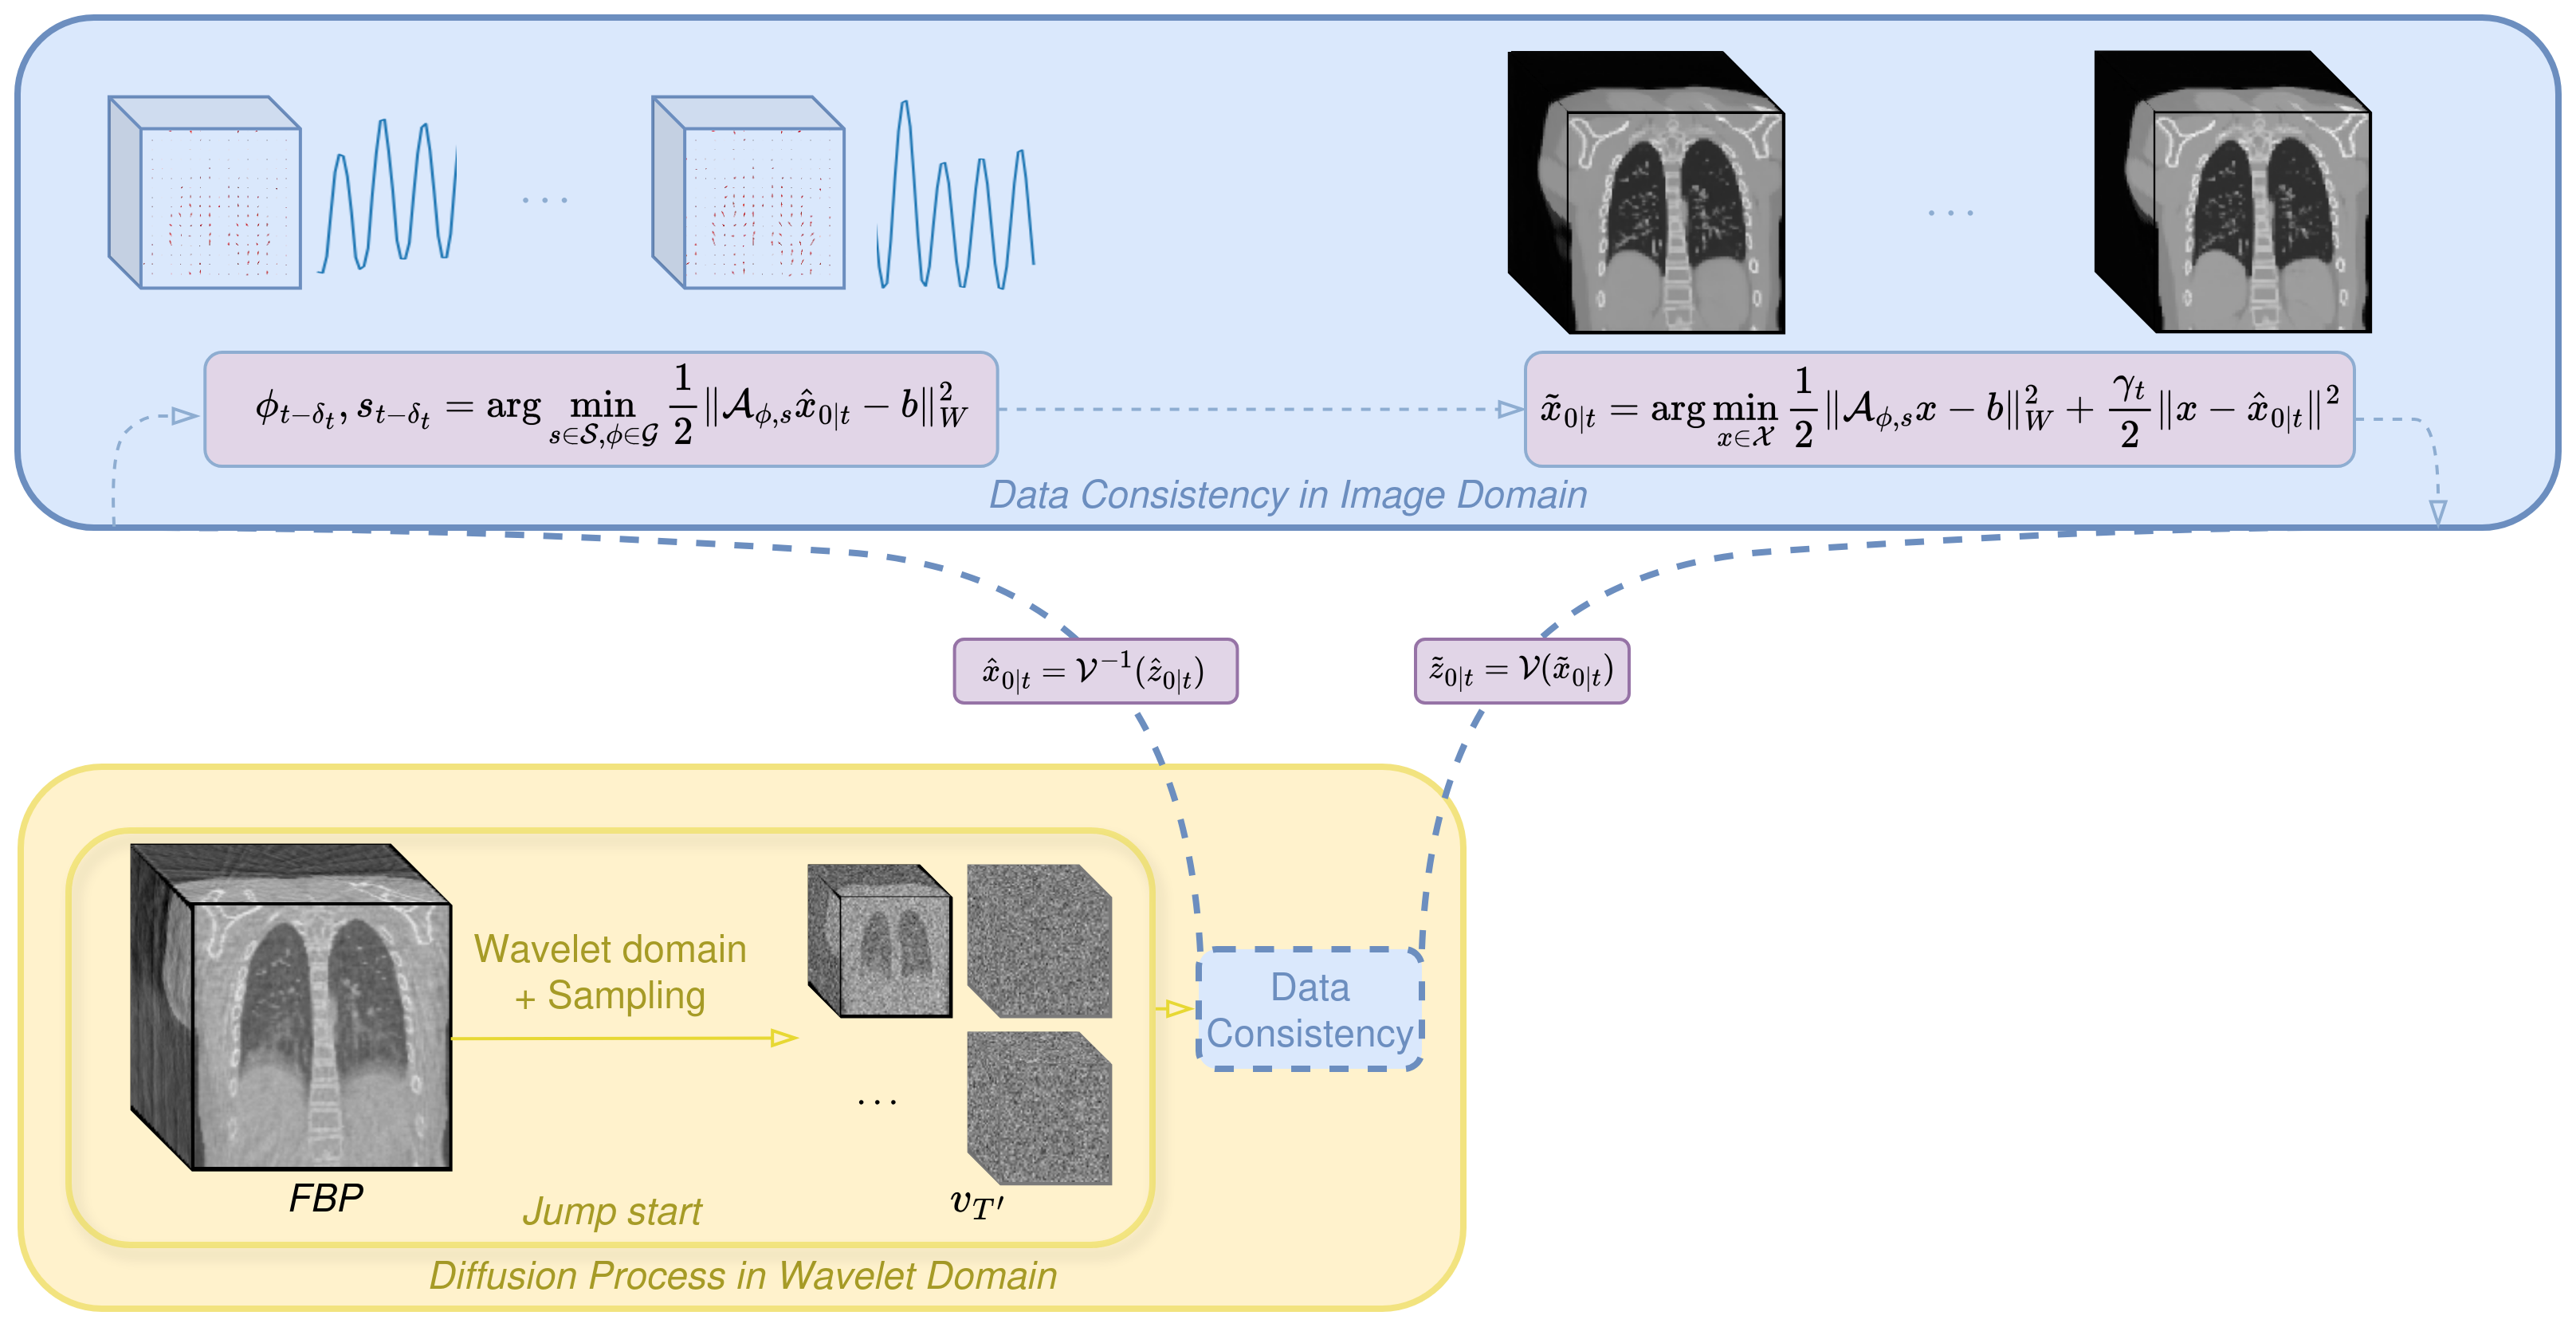
\includegraphics[width=1.0\linewidth]{figures/methods/overview/overview_4.png}}
        \only<5>{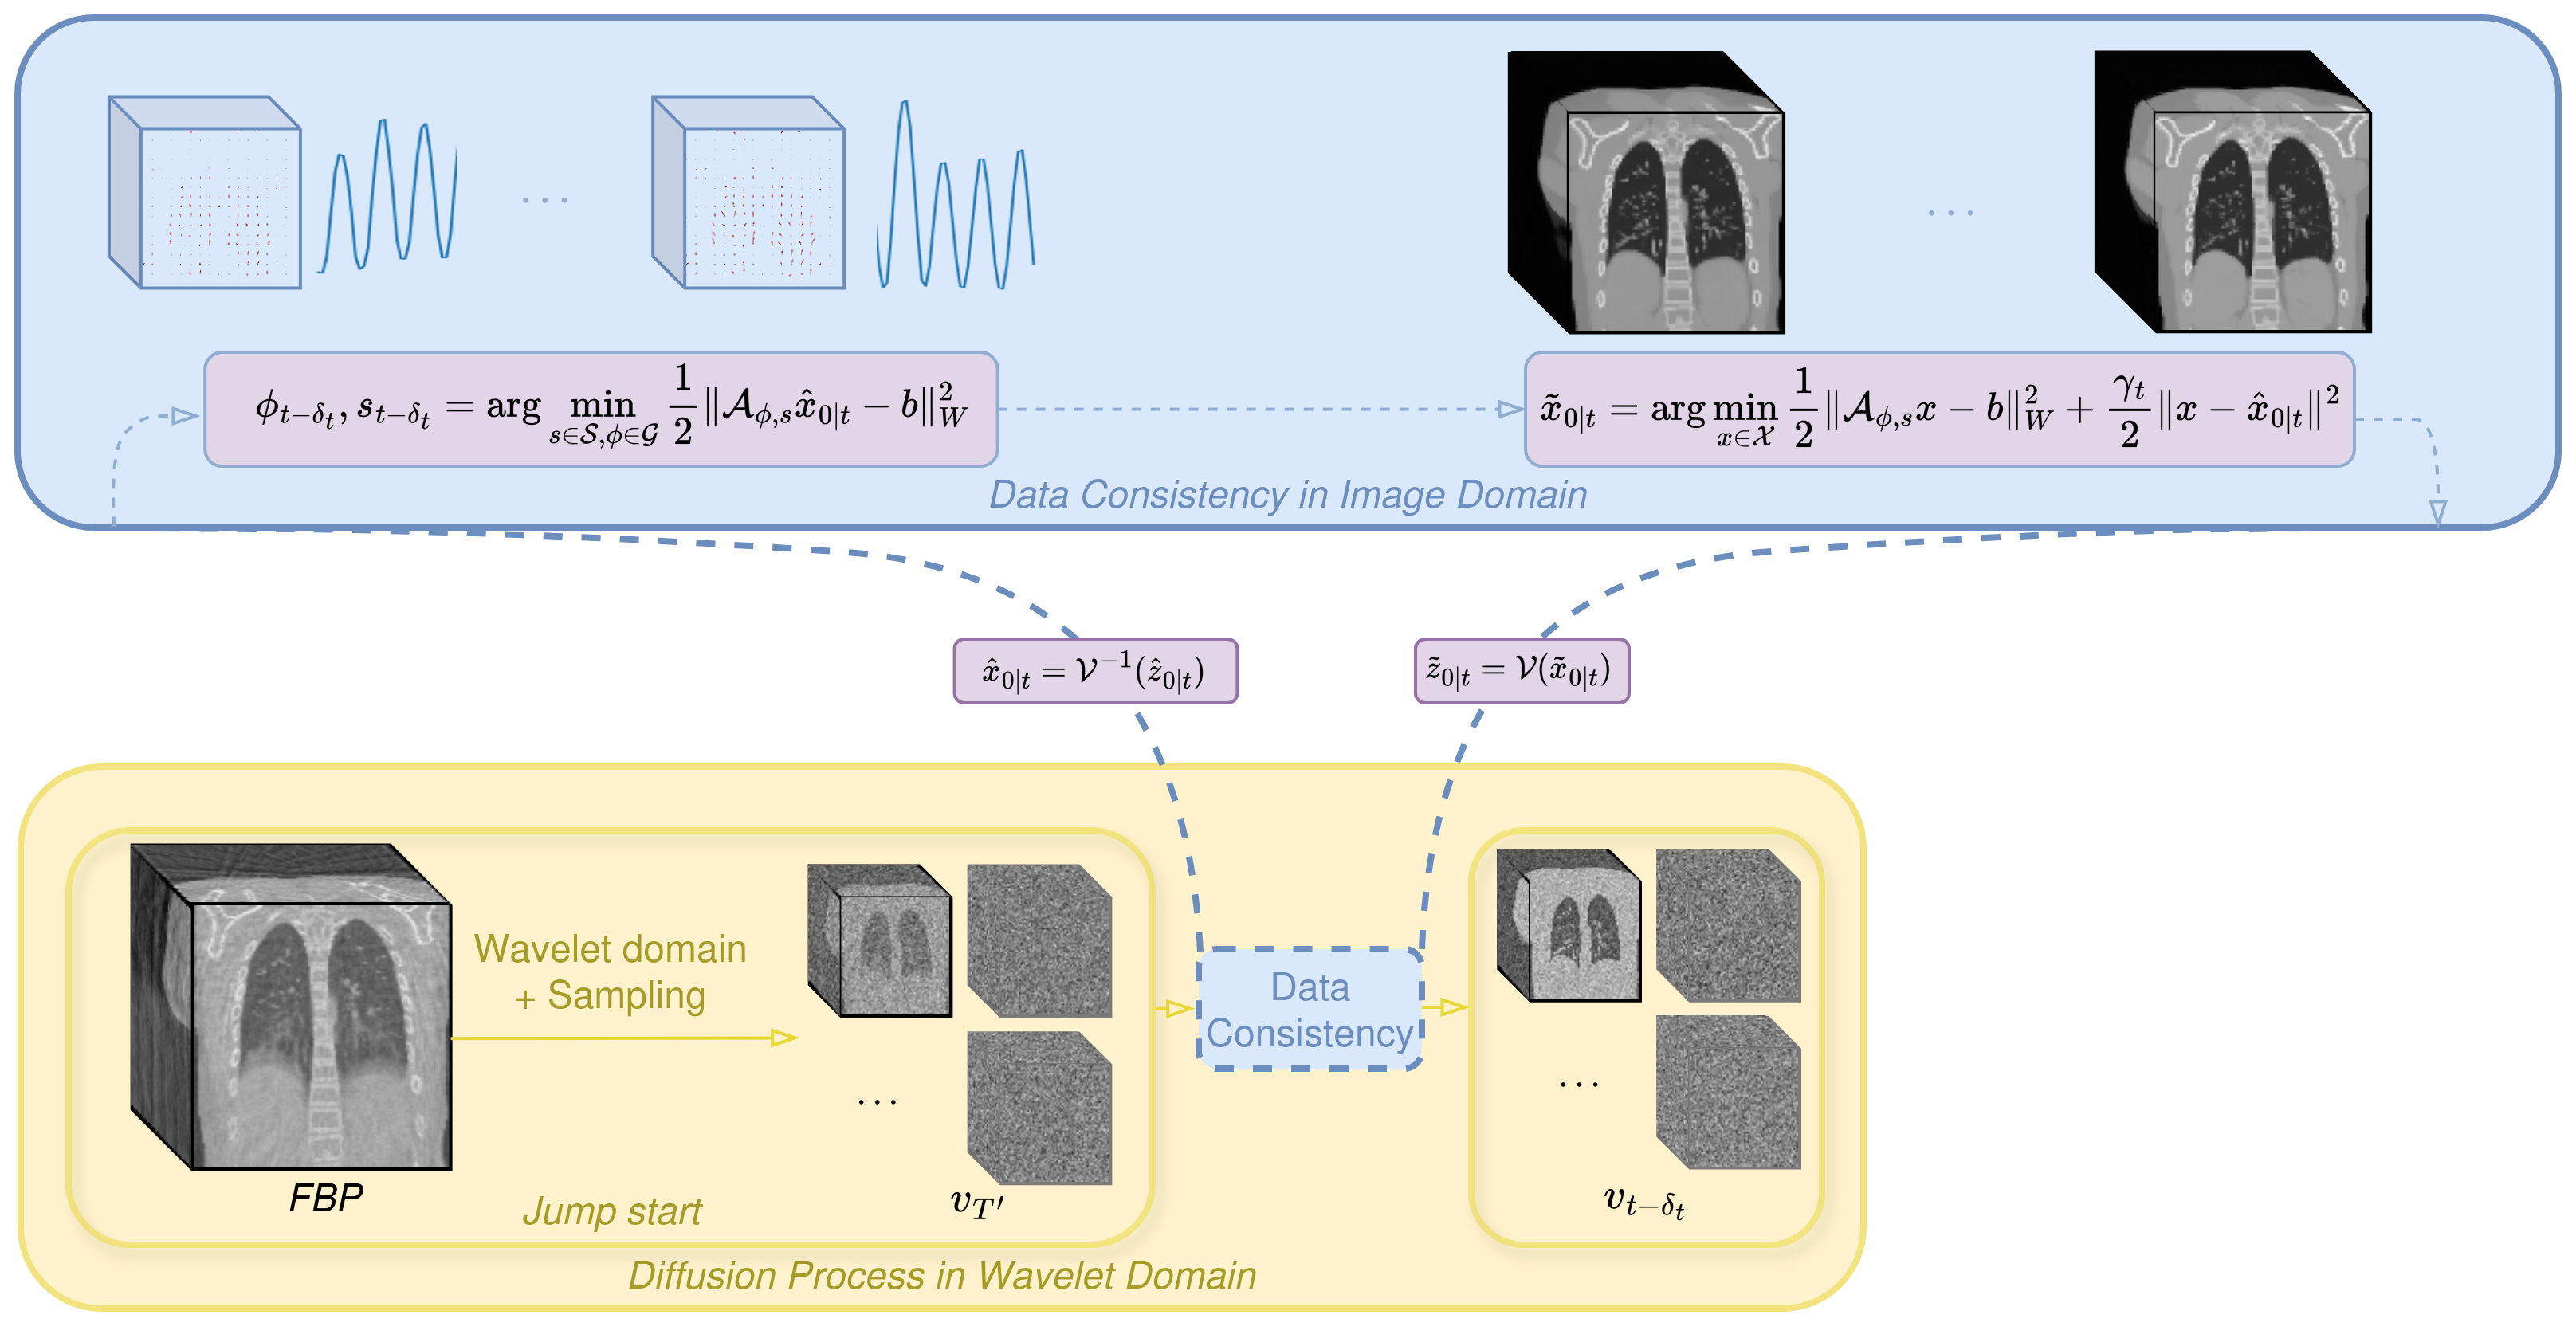
\includegraphics[width=1.0\linewidth]{figures/methods/overview/overview_5.png}}
        \only<6>{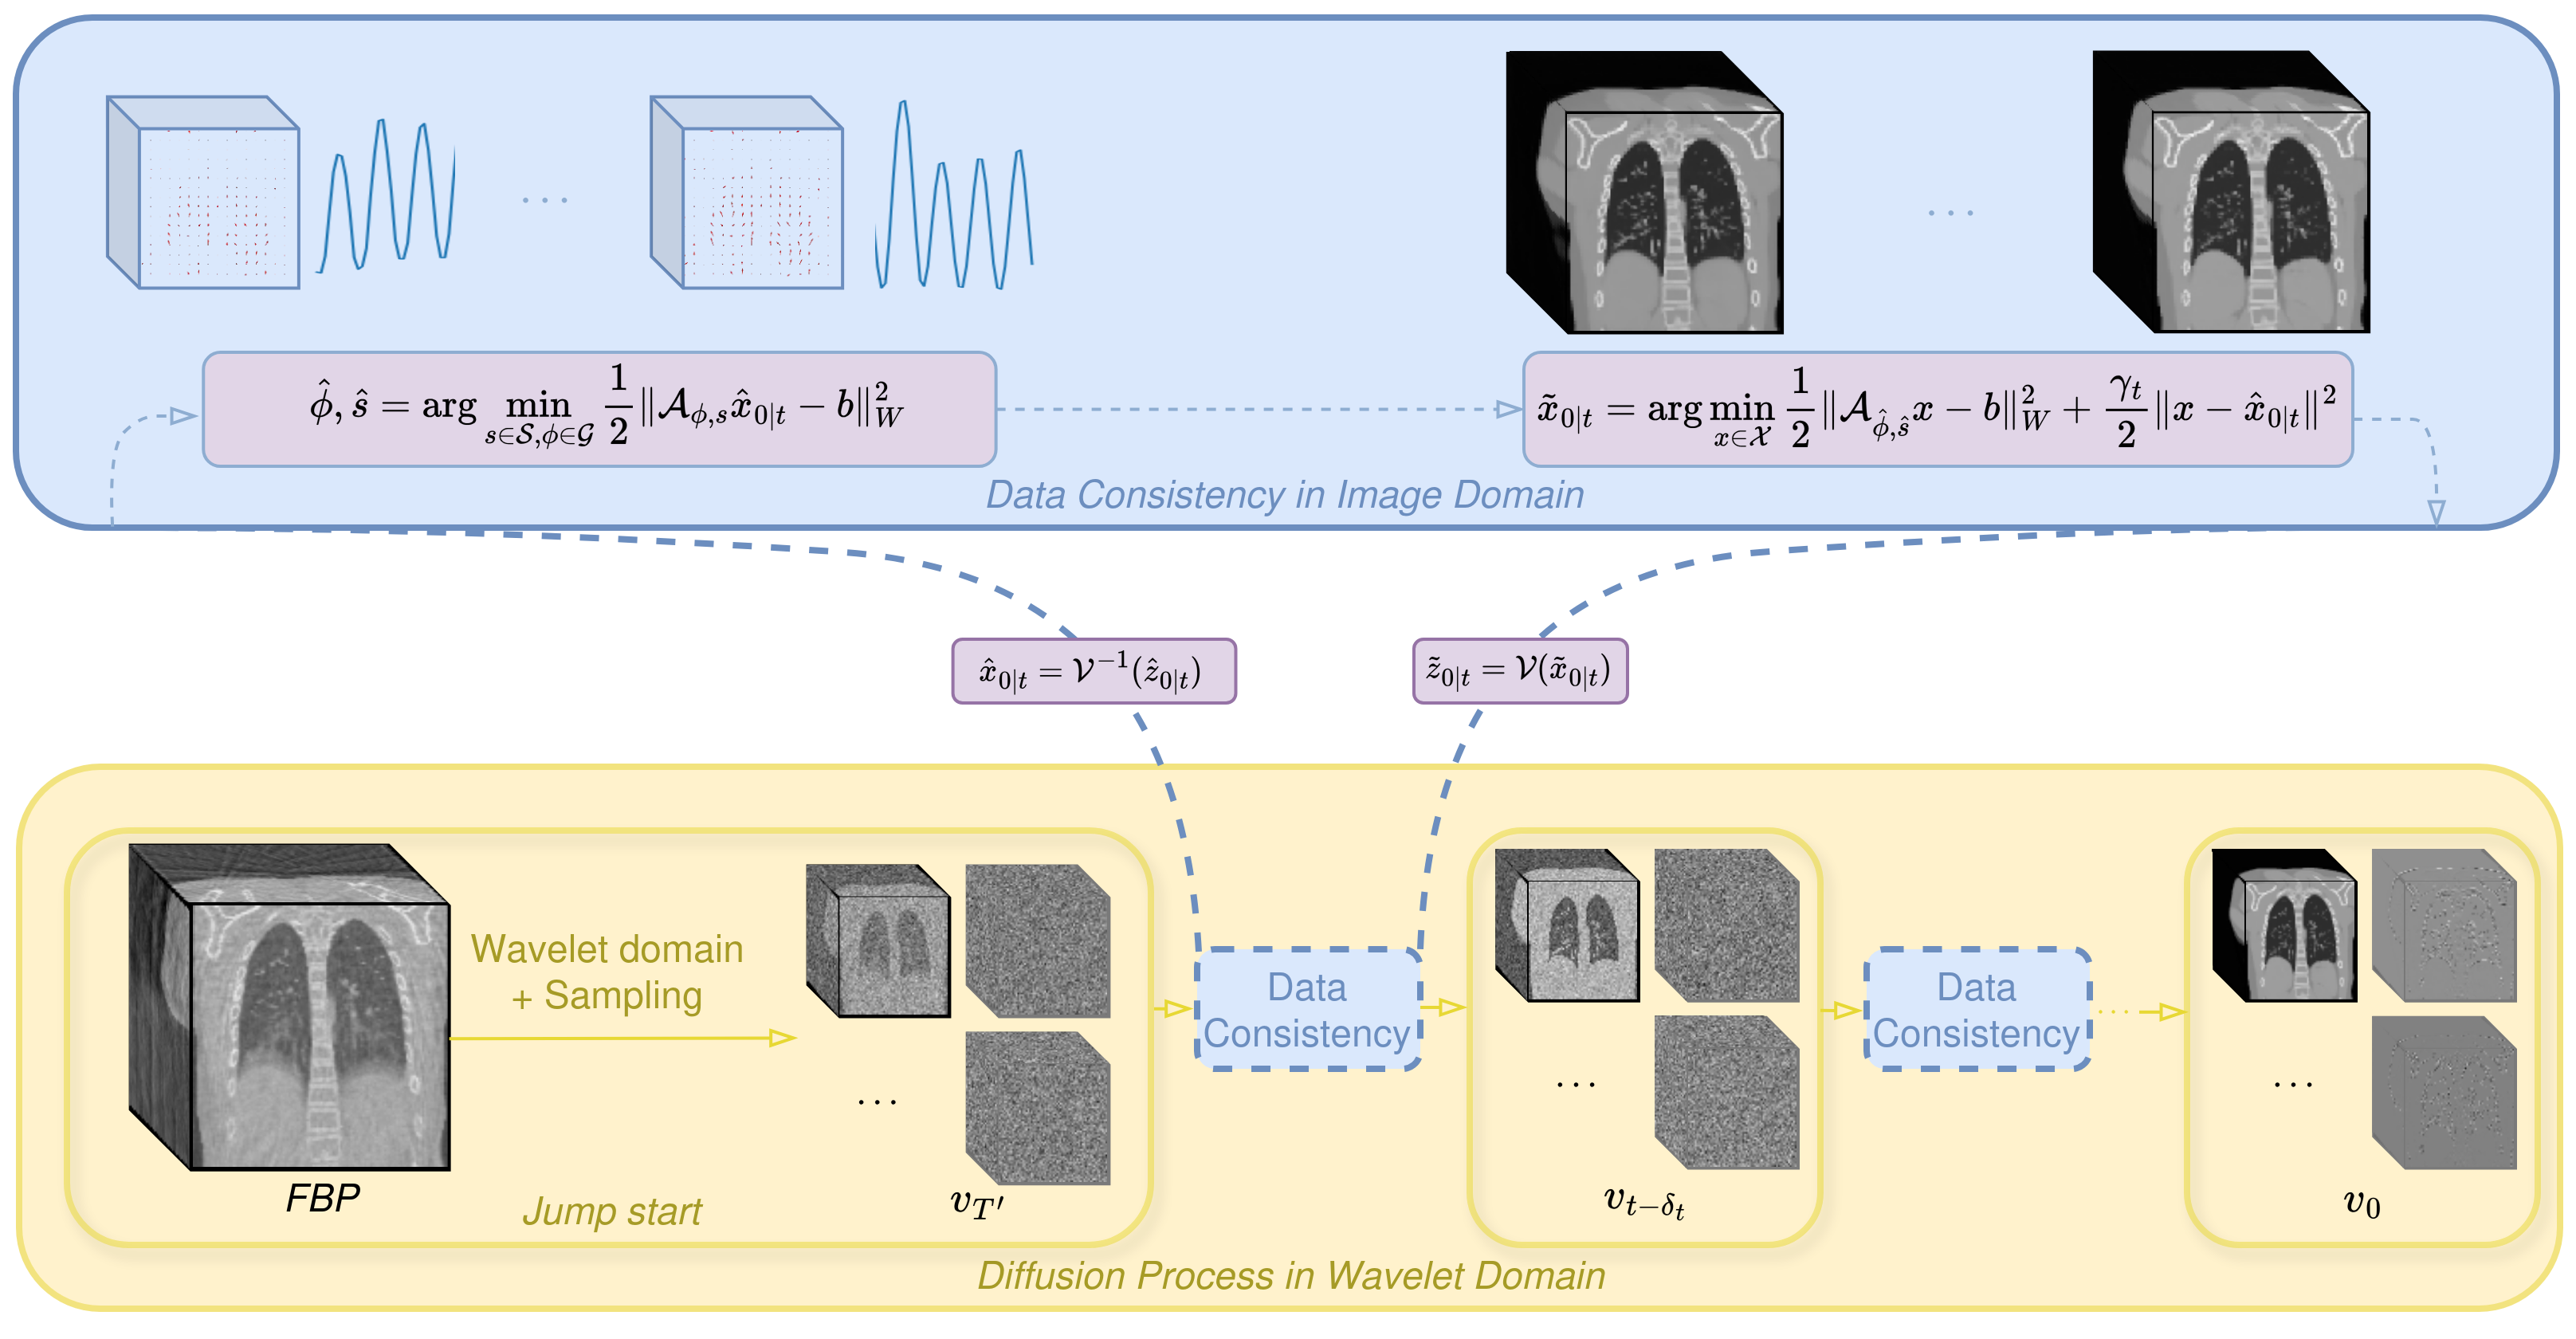
\includegraphics[width=1.0\linewidth]{figures/methods/overview/overview_6.png}}

\end{frame}